\section{Ejecucion}
\begin{itemize}
  \item A continuacion mostraremos la ejecucion de Videojuego.java en sus dos formas, la forma por consola, y la forma grafica
\end{itemize}
\subsection{Consola}
\begin{lstlisting}[language=bash, caption={Ejecucion del codigo por consola}]

===== Ejercito 1 =====
 Soldado 0x0:
  Nivel de vida: 3
  Fila: 9
  Columna: 1

 Soldado 0x1:
  Nivel de vida: 2
  Fila: 8
  Columna: 9

 Soldado 0x2:
  Nivel de vida: 5
  Fila: 3
  Columna: 9

 Soldado 0x3:
  Nivel de vida: 3
  Fila: 5
  Columna: 10

 Soldado 0x4:
  Nivel de vida: 1
  Fila: 7
  Columna: 1

 Soldado 0x5:
  Nivel de vida: 2
  Fila: 7
  Columna: 8

 Soldado 0x6:
  Nivel de vida: 4
  Fila: 8
  Columna: 8

 Soldado 0x7:
  Nivel de vida: 1
  Fila: 5
  Columna: 1


===== Ejercito 2 =====
 Soldado 1x0:
  Nivel de vida: 5
  Fila: 2
  Columna: 3

 Soldado 1x1:
  Nivel de vida: 1
  Fila: 10
  Columna: 9

 Soldado 1x2:
  Nivel de vida: 2
  Fila: 9
  Columna: 5

 Soldado 1x3:
  Nivel de vida: 3
  Fila: 2
  Columna: 9

 Soldado 1x4:
  Nivel de vida: 4
  Fila: 1
  Columna: 4

 Soldado 1x5:
  Nivel de vida: 1
  Fila: 2
  Columna: 2

 Soldado 1x6:
  Nivel de vida: 4
  Fila: 9
  Columna: 9

 Soldado 1x7:
  Nivel de vida: 1
  Fila: 5
  Columna: 4

 Soldado 1x8:
  Nivel de vida: 3
  Fila: 9
  Columna: 10

Soldado con maxima vida:
 Soldado 0x2:
  Nivel de vida: 5
  Fila: 3
  Columna: 9


===== Ranking de soldados: =====
 Soldado 0x4:
  Nivel de vida: 1
  Fila: 7
  Columna: 1

 Soldado 0x1:
  Nivel de vida: 2
  Fila: 8
  Columna: 9

 Soldado 0x5:
  Nivel de vida: 2
  Fila: 7
  Columna: 8

 Soldado 0x7:
  Nivel de vida: 1
  Fila: 5
  Columna: 1

 Soldado 0x0:
  Nivel de vida: 3
  Fila: 9
  Columna: 1

 Soldado 0x3:
  Nivel de vida: 3
  Fila: 5
  Columna: 10

 Soldado 0x6:
  Nivel de vida: 4
  Fila: 8
  Columna: 8

 Soldado 0x2:
  Nivel de vida: 5
  Fila: 3
  Columna: 9
\end{lstlisting}

\begin{itemize}
  \item A continuacion mostraremos la salida grafica del codigo
\end{itemize}
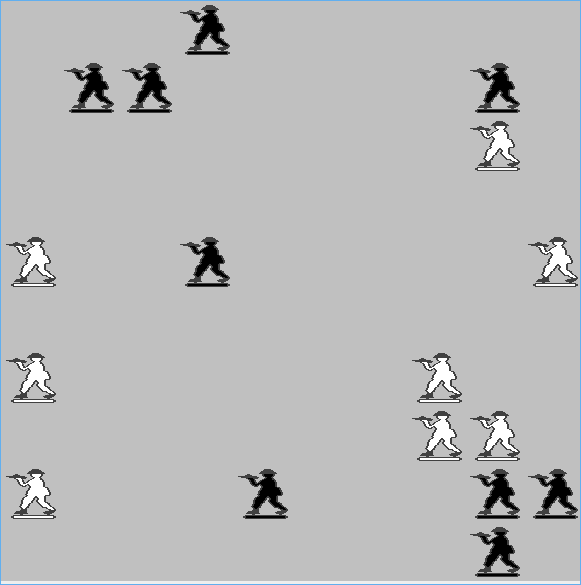
\includegraphics[width=0.5\textwidth] {img/salida.jpg}
